% -------------------------------------------------------------------------------- %

\begin{exercise}

\phantom{}

\begin{enumerate}[label = \textbf{\alph*)}]

  \item Es sei $\Omega = (0,1), t >0, f \in L^2(\Omega)$, und $X := H^1_D(\Omega) \times H^1_D(\Omega)$ mit $H^1_D(\Omega) := \Bbraces{u \in H^1(\Omega) | u(0) = 0}$.
  Das Problem des Timoshenko Balkens lautet:
  Gesucht ist $(w, \beta) \in X$ sodass für alle $(v, \delta) \in X$

  \begin{align}
    \Int[\Omega]{\beta^\prime \delta^\prime}{x}
    +
    \frac{1}{t^2} \Int[\Omega]{(w^\prime - \beta)(v^\prime - \delta)}{x}
    =
    \Int[\Omega]{f v}{x}.
  \end{align}

  Zeigen Sie, dass das Problem eindeutig lösbar ist. Wie verhält sich die Konstante in Cea's Lemma wenn $t \to 0$?
  \textit{Hinweis}:
  Verwenden Sie wie in Aufgabe 19 die Young Ungleichung für den gemischten Term sowie die Friedrich Ungleichung.

  \item Sei nun $\Omega \subset \R^2$ und $X := H^1_D(\Omega) \times [H^1_D(\Omega)]^2$.
  Betrachten Sie die Reissner-Mindlin Platte als zweidimiensionale Erweiterung des Timoshenko Balkens beschrieben durch das Problem:
  Gesucht ist $(w, \beta) \in X$ sodass für alle $(v, \delta) \in X$

  \begin{align}
    \Int[\Omega]{\epsilon(\beta):\epsilon(\delta)}{x}
    +
    \frac{1}{t^2} \Int[\Omega]{(\nabla w - \beta) \cdot (\nabla v - \delta)}{x}
    =
    \Int[\Omega]{f v}{x},
  \end{align}

  wobei $\epsilon(\beta) := 0.5 (\nabla \beta + (\nabla \beta)^\top)$ der symmetrische Gradient ist.
  Untersuchen Sie mit dem zur Verfügung gestellten Jupyter-File das Konvergenzverhalten für lineare Elemente bei verschiedenen Dickenparametern, $t \in \Bbraces{1, 0.1, 0.01, 0.001}$.
  Was beobachten Sie?
  Wie ändert sich das Verhalten für quadratisch finite Elemente?

\end{enumerate}

\end{exercise}

% -------------------------------------------------------------------------------- %

\begin{solution}

\phantom{}

\begin{enumerate}[label = \textbf{\alph*)}]

  \item Wir wollen wieder Exercise 7 (Lemma of Lax-Milgram) anwenden, diesmal mit

  \begin{align*}
    a
    \pbraces
    {
      \begin{pmatrix}
        w \\ \beta
      \end{pmatrix},
      \begin{pmatrix}
        v \\ \delta
      \end{pmatrix}
    }
    :=
    \Int[\Omega]{\beta^\prime \delta^\prime}{x}
    +
    \frac{1}{t^2} \Int[\Omega]{(w^\prime - \beta)(v^\prime - \delta)}{x},
    \quad
    F
    \begin{pmatrix}
      v \\ \delta
    \end{pmatrix}
    :=
    \Int[\Omega]{f v}{x}.
  \end{align*}

  \begin{enumerate}[label = \arabic*.]

    \item Schritt (Stetigkeit von $a$):

    Auf dem $\R^2$ sind die Normen $\norm[1]{\cdot}$ und $\norm[2]{\cdot}$ äquivalent.
    Wir erhalten also eine Konstante $C > 0$, sodass $\norm[1]{\cdot} \leq C \norm[2]{\cdot}$.

    \begin{align*}
      \norm[1]{\cdot}
      \sim
      \norm[2]{\cdot}
      ~\text{auf $\R^2$}~
      \implies
      \Exists C > 0:
      \norm[1]{\cdot}
      \leq
      C
      \norm[2]{\cdot}
    \end{align*}

    Vorausschauend auf das Lemma 1.6 (Céa), definieren wir noch die Konstante

    \begin{align*}
      \beta_t
      :=
      \max \Bbraces{1, \frac{1}{t^2}} C.
    \end{align*}

    \begin{align*}
      a
      \pbraces
      {
        \begin{pmatrix}
          w \\ \beta
        \end{pmatrix},
        \begin{pmatrix}
          v \\ \delta
        \end{pmatrix}
      }
      & =
      \Int[\Omega]{\beta^\prime \delta^\prime}{x}
      +
      \frac{1}{t^2} \Int[\Omega]{(w^\prime - \beta)(v^\prime - \delta)}{x} \\
      & \stackrel
      {
        \mathrm{CSB}
      }{\leq}
      \norm[L^2(\Omega)]{\beta^\prime}
      \norm[L^2(\Omega)]{\delta^\prime}
      +
      \frac{1}{t^2}
      \norm[L^2(\Omega)]{w^\prime - \beta}
      \norm[L^2(\Omega)]{v^\prime - \delta} \\
      & \leq
      \norm[L^2(\Omega)]{\beta^\prime}
      \norm[L^2(\Omega)]{\delta^\prime}
      +
      \frac{1}{t^2}
      \pbraces
      {
        \norm[L^2(\Omega)]{w^\prime} +
        \norm[L^2(\Omega)]{\beta}
      }
      \pbraces
      {
        \norm[L^2(\Omega)]{v^\prime} +
        \norm[L^2(\Omega)]{\delta}
      } \\
      & \leq
      \max \Bbraces{1, \frac{1}{t^2}}
      \pbraces
      {
        \norm[L^2(\Omega)]{w^\prime} +
        \norm[H^1(\Omega)]{\beta}
      }
      \pbraces
      {
        \norm[L^2(\Omega)]{v^\prime} +
        \norm[H^1(\Omega)]{\delta}
      } \\
      & \leq \cdots \leq
      \max \Bbraces{1, \frac{1}{t^2}} C
      \pbraces
      {
        \norm[H^1(\Omega)]{w}^2 +
        \norm[H^1(\Omega)]{\beta}^2
      }^{1/2}
      \pbraces
      {
        \norm[H^1(\Omega)]{v}^2 +
        \norm[H^1(\Omega)]{\delta}^2
      }^{1/2} \\
      & =
      \beta_t
      \norm[X]
      {
        \begin{pmatrix}
          w \\ \beta
        \end{pmatrix}
      }
      \norm[X]
      {
        \begin{pmatrix}
          v \\ \delta
        \end{pmatrix}
      }
    \end{align*}

    \item Schritt (Elliptizität von $a$):

    \begin{enumerate}[label = \arabic*.]

      \item Hilfs-Ungleichung (Friedrich):

      \begin{center}
        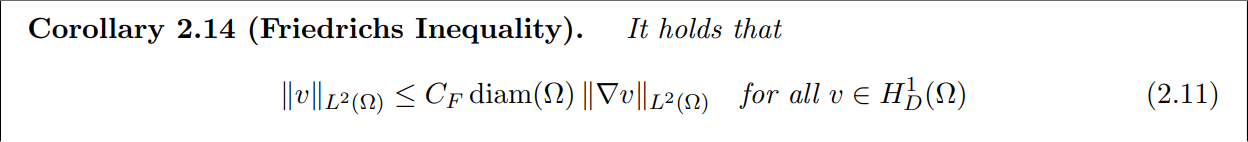
\includegraphics[width = 0.75 \textwidth]{NumPDEs/NumPDEs - Corollary 2.14.1 (Friedrichs Inequality).png} \\
        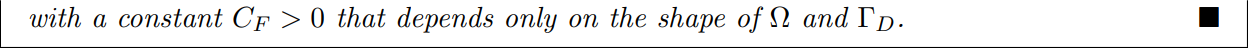
\includegraphics[width = 0.75 \textwidth]{NumPDEs/NumPDEs - Corollary 2.14.2 (Friedrichs Inequality).png}
      \end{center}

      \begin{align*}
        \implies
        \norm[H^1(\Omega)]{v}^2
        =
        \norm[L^2(\Omega)]{v}
        +
        \norm[L^2(\Omega)]{\nabla v}
        \stackrel
        {
          \mathrm{F}
        }{\leq}
        (
          C_F
          \underbrace{\diam \Omega}_1
          +
          1
        )^2
        \norm[L^2(\Omega)]{v^\prime}^2
      \end{align*}

      \item Hilfs-Ungleichung (Young):

      Dabei wollen wir $\varepsilon_t$ wie folgt wählen.

      \begin{align*}
        \varepsilon_t
        \in
        \pbraces
        {
          \frac{1}
          {
            1
            +
            \frac{t^2}{(C_F + 1)^2}
          },
          1
        }
        \neq
        \emptyset
      \end{align*}

      Das Intervall ist dabei nicht die leere Menge, weil $t > 0$ und daher

      \begin{align*}
        1 < 1 + \frac{t^2}{(C_F + 1)^2}.
      \end{align*}

    \end{enumerate}

    Vorausschauend auf das Lemma 1.6 (Céa), definieren wir noch die Konstante

    \begin{align*}
      \alpha_t
      :=
      \min
      \Bbraces
      {
        \frac{1}{(C_F + 1)^2}
        +
        \frac{1}{t^2}
        \pbraces
        {
          1 - \frac{1}{\varepsilon_t}
        },
        \frac
        {
          1 - \varepsilon_t
        }{
          t^2 (C_F + 1)^2
        }
      }.
    \end{align*}

    \begin{align*}
      a
      \pbraces
      {
        \begin{pmatrix}
          w \\ \beta
        \end{pmatrix},
        \begin{pmatrix}
          w \\ \beta
        \end{pmatrix}
      }
      & =
      \norm[L^2(\Omega)]{\beta^\prime}^2
      +
      \frac{1}{t^2}
      \Int[\Omega]{\abs{w^\prime - \beta}^2}{x} \\
      & =
      \norm[L^2(\Omega)]{\beta^\prime}^2
      +
      \frac{1}{t^2}
      \pbraces
      {
        \norm[L^2(\Omega)]{w^\prime}^2
        +
        \Int[\Omega]{- 2 w^\prime \beta}{x}
        +
        \norm[L^2(\Omega)]{\beta}^2
      } \\
      & \stackrel
      {
        \mathrm{Y}
      }{\geq}
      \norm[L^2(\Omega)]{\beta^\prime}^2
      +
      \frac{1}{t^2}
      \pbraces
      {
        \norm[L^2(\Omega)]{w^\prime}^2
        +
        \Int[\Omega]{- \varepsilon_t \abs{w^\prime}^2}{x}
        +
        \Int[\Omega]{- \frac{1}{\varepsilon_t} \abs{\beta}^2}{x}
        +
        \norm[L^2(\Omega)]{\beta}^2
      } \\
      & =
      \norm[L^2(\Omega)]{\beta^\prime}^2
      +
      \frac{1}{t^2}
      \pbraces
      {
        (1 - \varepsilon_t)
        \norm[L^2(\Omega)]{w^\prime}^2
        +
        \pbraces
        {
          1 - \frac{1}{\varepsilon_t}
        }
        \norm[L^2(\Omega)]{\beta}^2
      } \\
      & \stackrel
      {
        \mathrm{F}
      }{\geq}
      \frac{1}{(C_F + 1)^2}
      \norm[H^1(\Omega)]{\beta}^2
      +
      \frac{1}{t^2}
      \pbraces
      {
        \frac{1 - \varepsilon_t}{(C_F + 1)^2}
        \norm[H^1(\Omega)]{w}^2
        +
        \pbraces
        {
          1 - \frac{1}{\varepsilon_t}
        }
        \norm[H^1(\Omega)]{\beta}^2
      } \\
      & =
      \pbraces
      {
        \frac{1}{(C_F + 1)^2}
        +
        \frac{1}{t^2}
        \pbraces
        {
          1 - \frac{1}{\varepsilon_t}
        }
      }
      \norm[H^1(\Omega)]{\beta}^2
      +
      \frac{1 - \varepsilon_t}{t^2 (C_F + 1)^2}
      \norm[H^1(\Omega)]{w}^2 \\
      & \geq
      \min
      \Bbraces
      {
        \frac{1}{(C_F + 1)^2}
        +
        \frac{1}{t^2}
        \pbraces
        {
          1 - \frac{1}{\varepsilon_t}
        },
        \frac
        {
          1 - \varepsilon_t
        }{
          t^2 (C_F + 1)^2
        }
      }
      \pbraces
      {
        \norm[H^1(\Omega)]{w}^2
        +
        \norm[H^1(\Omega)]{\beta}^2
      } \\
      & =
      \alpha_t
      \norm[X]
      {
        \begin{pmatrix}
          w \\ \beta
        \end{pmatrix}
      }^2
    \end{align*}

    \item Schritt (Stetigkeit von $F$):

    \begin{align*}
      F
      \begin{pmatrix}
        v \\ \delta
      \end{pmatrix}
      =
      \Int[\Omega]{f v}{x}
      \stackrel
      {
        \mathrm{CSB}
      }{\leq}
      \norm[L^2(\Omega)]{f}
      \norm[L^2(\Omega)]{v}
      \leq
      \norm[L^2(\Omega)]{f}
      \norm[X]
      {
        \begin{pmatrix}
          v \\ \delta
        \end{pmatrix}
      }
    \end{align*}

  \end{enumerate}

  \includegraphicsunboxed{NumPDEs/NumPDEs - Lemma 1.6 (Céa).png}

  Der Quotient in Lemma 1.6 (Céa) divergiert.

  \begin{align*}
    \beta_t
    & =
    \max \Bbraces{1, \frac{1}{t^2}} C
    \xrightarrow{t \to 0}
    \infty, \\
    \alpha_t
    & =
    \min
    \Bbraces
    {
      \frac{1}{(C_F + 1)^2}
      +
      \frac{1}{t^2}
      \pbraces
      {
        1 - \frac{1}{\varepsilon_t}
      },
      \frac
      {
        1 - \varepsilon_t
      }{
        t^2 (C_F + 1)^2
      }
    }
    \leq
    \frac
    {
      1 - \varepsilon_t
    }{
      t^2 (C_F + 1)^2
    }
    \leq
    \frac
    {
      1
      -
      \frac{1}
      {
        1
        +
        \frac{t^2}{(C_F + 1)^2}
      }
    }{
      t^2 (C_F + 1)^2
    } \\
    & =
    \frac
    {
      1 + \frac{t^2}{(C_f + 1)^2} - 1
    }{
      \pbraces
      {
        1 + \frac{t^2}{(C_F + 1)^2}
      }
      t^2 (C_F + 1)^2
    }
    =
    \frac{1}
    {
      (C_F + 1)^2
      \pbraces
      {
        (C_F + 1)^2 + t^2
      }
    }
    \xrightarrow{t \to 0}
    \frac{1}{(C_F + 1)^4} \\
    \implies
    \frac{\beta_t}{\alpha_t}
    & \xrightarrow{t \to 0}
    \infty
  \end{align*}

  Die Fehlerschranke (d.h. die rechte Seite von (1.20)) kann also beliebig groß werden.
  Somit können wir Lemma 1.6 (Céa) nicht anwenden, um den FEM-Fehler sinnvoll abzuschätzen.

\end{enumerate}

\end{solution}

% -------------------------------------------------------------------------------- %
